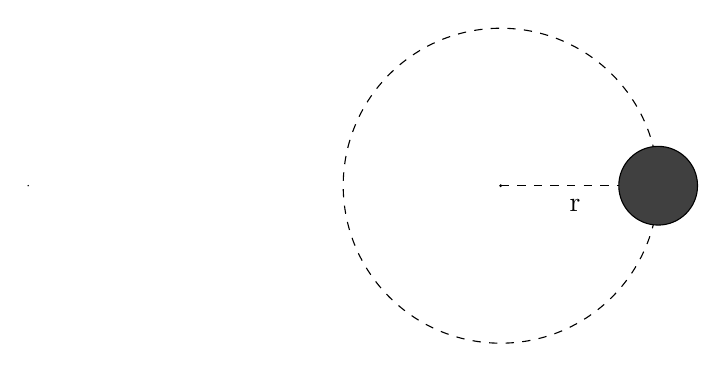
\begin{tikzpicture}
\draw[black] (0,0) circle (0.0001cm);
\draw[dashed, draw=black] (6,0) circle (2cm);
\draw[dashed, draw=black] (6,0) circle (0.01cm);
\draw[dashed, black] (6,0) -- (8,0);
\draw[black] (6.75,-0.25) node[anchor=west] {r};
\filldraw[fill = darkgray, draw=black] (8,0) circle (0.5cm);
\end{tikzpicture}
\newline

Now that we have dealt with linear motion, we need to deal with centripetal(circular) motion. There are only a few things you need to know about centripetal forces, but once you know the first few things, we will be able to do quite a lot. The first thing you need to know is when we can talk about centripetal force, motion, and acceleration. We should discuss centripetal motion when an object is moving in a circle. We do not want to think about centripetal force in the same way here as when an object is rotating about an axis inside of it. For example, if we think about the earth circularly going around the sun, we can discuss centripetal force. Meanwhile, if we think about a fidget spinner rotating around its center, we can not think about centripetal force. However, if we were to think about one small slice of one blade of the fidget spinner moving about in a circle, we could think about centripetal force. Hopefully, these examples will give you the idea. Later, we will discuss rotational motion, and as you will see, there are connections between rotational and centripetal motion, as essentially, they describe the same concepts.

Next, we need to think about what centripetal motion we will study entails. For us, centripetal motion is when an object is rotating around in a circle with a constant speed. So, what is different about centripetal motion compared to accelerating linear motion is that centripetal motion involves the magnitude of velocity(speed), staying constant, while the direction of the velocity is changing. This means that $\frac{dv}{dt}$ is not zero, because $\vec{v}$ is a vector and its direction is changing. Next, we need to think about the magnitude of the acceleration that is being produced in addition to the direction of the acceleration that is being produced. I am going to spare the details of the proof here because I believe they involve more mathematics than physics. However, I would still recommend you search for the proof yourself because it is beneficial to know exactly why this formula is true because it is ubiquitous. The formula is that \begin{equation}a_c=\frac{v^2}{r}\end{equation} with $a_c$ representing the magnitude of the centripetal acceleration and $r$ being the radius of the circle that is formed by the movement of the object. You also need to know that the centripetal acceleration is directed directly towards the center of the circle that the object is moving around. I am going to give a sort of proof by contradiction as to why this is true. First, remember that the velocity of an object moving around in a circle is directly tangent to the point along the circle that the object is in. This is because the velocity of an object must always be tangent to the path of its motion, by definition. Next, imagine that the acceleration had a component in the direction tangent to the circle. Then, the velocity of the object would increase or decrease. But we have said that the velocity of the object is remaining the same when undergoing centripetal acceleration. This is a contradiction. So all of the centripetal acceleration must be pointed towards the center of the object's path. This direction is called the radial direction. Now that we have an understanding of the direction of the centripetal acceleration, we should try to justify why the formula would be true physically. First, let us think about why $a_c$ should be larger when we have a larger velocity. This is because if the velocity is higher, a larger acceleration is required to switch the direction of the velocity faster(assuming a constant radius). Next, we need to think about why increasing the radius would decrease the centripetal acceleration. This is because when we have a larger radius, the object “has more time” to modify its velocity. If you are not satisfied by these explanations(as I was at first), I recommend you go through the mathematical derivation which should only serve to strengthen your physical intuition. 
Now that we know the formula for centripetal acceleration, we need to understand how it applies. You may be having a question now, what even is centripetal acceleration? Well, essentially, centripetal acceleration is the acceleration in the inward radial direction that is required for an object to go into a circle. So essentially, it is a real requirement, but forces do not cause a centripetal acceleration only. This sounds kind of silly so let us go through a real example to strengthen this idea. 

The classic example is a block on a string that is swirling in a circle in a vertical plane. Imagine that the string is the black line and that the rightmost endpoint of the string is being held constant in space such that the entire string is rotating in a circle. Let me give you a challenge now. If we say that the object has a mass m, is in rotation at a constant velocity of v in the plane with a circular trajectory of radius r, what is the value of the tension in the string holding the object as a function of the angle $\theta$(you only need to do this when the mass is above the rightmost end of the string and to the left of the center of the string)? The AP Exam will probably only ask you about this at the highest and lowest points of the circular trajectory of the mass, so I recommend that you find these as well. 

Now that you have either solved the problem or if you can’t seem to figure it out, let us use Newton’s laws to solve this problem. Remember that the direction of the centripetal acceleration is always vertically inward(which the tension also is, and which a component of the force of gravity is. We discussed how to find the component of the force of gravity earlier, so I will not discuss it here and recommend that you go back to the slanted plane lesson earlier to see this discussion. We have that the component of the force of gravity in the inward radial direction is $$mg\sin\left(\theta \right)$$ So we need to add the gravity and tension together to find the total force on the object in the inward radial direction, we find that \begin{equation}T+mg\sin\left(\theta \right)=F_c\end{equation} But $F_c=ma_c$, and $a_c=\frac{v^2}{r}$. because the direction of the centripetal acceleration behaves like any other direction in the eyes of nature. So we have that \begin{equation}T=\frac{mv^2}{r}-mg\sin\left(\theta \right)\end{equation} That is our entire expression because everything is constant other than $\theta$. Hopefully, this example showed how to deal with forces so we can use our formula for centripetal acceleration to our advantage. 